% Options for packages loaded elsewhere
\PassOptionsToPackage{unicode}{hyperref}
\PassOptionsToPackage{hyphens}{url}
%
\documentclass[
]{article}
\usepackage{amsmath,amssymb}
\usepackage{lmodern}
\usepackage{iftex}
\ifPDFTeX
  \usepackage[T1]{fontenc}
  \usepackage[utf8]{inputenc}
  \usepackage{textcomp} % provide euro and other symbols
\else % if luatex or xetex
  \usepackage{unicode-math}
  \defaultfontfeatures{Scale=MatchLowercase}
  \defaultfontfeatures[\rmfamily]{Ligatures=TeX,Scale=1}
\fi
% Use upquote if available, for straight quotes in verbatim environments
\IfFileExists{upquote.sty}{\usepackage{upquote}}{}
\IfFileExists{microtype.sty}{% use microtype if available
  \usepackage[]{microtype}
  \UseMicrotypeSet[protrusion]{basicmath} % disable protrusion for tt fonts
}{}
\makeatletter
\@ifundefined{KOMAClassName}{% if non-KOMA class
  \IfFileExists{parskip.sty}{%
    \usepackage{parskip}
  }{% else
    \setlength{\parindent}{0pt}
    \setlength{\parskip}{6pt plus 2pt minus 1pt}}
}{% if KOMA class
  \KOMAoptions{parskip=half}}
\makeatother
\usepackage{xcolor}
\IfFileExists{xurl.sty}{\usepackage{xurl}}{} % add URL line breaks if available
\IfFileExists{bookmark.sty}{\usepackage{bookmark}}{\usepackage{hyperref}}
\hypersetup{
  pdftitle={A multi-stock, multi-region state-space age-structured assessment model with an application to black sea bass},
  pdfauthor={Timothy J. Miller1; Kierstin Curti; Alex Hansell},
  hidelinks,
  pdfcreator={LaTeX via pandoc}}
\urlstyle{same} % disable monospaced font for URLs
\usepackage[margin=1in]{geometry}
\usepackage{graphicx}
\makeatletter
\def\maxwidth{\ifdim\Gin@nat@width>\linewidth\linewidth\else\Gin@nat@width\fi}
\def\maxheight{\ifdim\Gin@nat@height>\textheight\textheight\else\Gin@nat@height\fi}
\makeatother
% Scale images if necessary, so that they will not overflow the page
% margins by default, and it is still possible to overwrite the defaults
% using explicit options in \includegraphics[width, height, ...]{}
\setkeys{Gin}{width=\maxwidth,height=\maxheight,keepaspectratio}
% Set default figure placement to htbp
\makeatletter
\def\fps@figure{htbp}
\makeatother
\setlength{\emergencystretch}{3em} % prevent overfull lines
\providecommand{\tightlist}{%
  \setlength{\itemsep}{0pt}\setlength{\parskip}{0pt}}
\setcounter{secnumdepth}{5}
\newlength{\cslhangindent}
\setlength{\cslhangindent}{1.5em}
\newlength{\csllabelwidth}
\setlength{\csllabelwidth}{3em}
\newlength{\cslentryspacingunit} % times entry-spacing
\setlength{\cslentryspacingunit}{\parskip}
\newenvironment{CSLReferences}[2] % #1 hanging-ident, #2 entry spacing
 {% don't indent paragraphs
  \setlength{\parindent}{0pt}
  % turn on hanging indent if param 1 is 1
  \ifodd #1
  \let\oldpar\par
  \def\par{\hangindent=\cslhangindent\oldpar}
  \fi
  % set entry spacing
  \setlength{\parskip}{#2\cslentryspacingunit}
 }%
 {}
\usepackage{calc}
\newcommand{\CSLBlock}[1]{#1\hfill\break}
\newcommand{\CSLLeftMargin}[1]{\parbox[t]{\csllabelwidth}{#1}}
\newcommand{\CSLRightInline}[1]{\parbox[t]{\linewidth - \csllabelwidth}{#1}\break}
\newcommand{\CSLIndent}[1]{\hspace{\cslhangindent}#1}
\usepackage{url}
\usepackage{setspace}
%\singlespacing
%\onehalfspacing
\doublespacing
\usepackage{lineno}
\linenumbers
\usepackage[belowskip=0pt,aboveskip=0pt]{caption}
\usepackage{relsize}
\usepackage{float}
% \usepackage[section]{placeins}
\usepackage{lscape}
\usepackage{longtable}
\usepackage{amsmath,rotating}
\usepackage[scanall]{psfrag}
\usepackage{bm}
\usepackage{caption,graphics}
\usepackage{graphicx}
%\usepackage{natbib}
%\usepackage[nottoc]{tocbibind}
%\usepackage{indentfirst}
\usepackage{sectsty}
\usepackage{color}
\usepackage{fancyhdr}
\usepackage{xspace}
\usepackage{textcomp}
\usepackage{upgreek}

\newcommand{\blandscape}{\begin{landscape}}
\newcommand{\elandscape}{\end{landscape}}
\usepackage{booktabs}
\usepackage{longtable}
\usepackage{array}
\usepackage{multirow}
\usepackage{wrapfig}
\usepackage{float}
\usepackage{colortbl}
\usepackage{pdflscape}
\usepackage{tabu}
\usepackage{threeparttable}
\usepackage{threeparttablex}
\usepackage[normalem]{ulem}
\usepackage{makecell}
\usepackage{xcolor}
\ifLuaTeX
  \usepackage{selnolig}  % disable illegal ligatures
\fi

\title{A multi-stock, multi-region state-space age-structured assessment
model with an application to black sea bass}
\author{Timothy J. Miller\textsuperscript{1} \and Kierstin
Curti \and Alex Hansell}
\date{16 September, 2024}

\begin{document}
\maketitle

\(^1\)\href{mailto:timothy.j.miller@noaa.gov}{\nolinkurl{timothy.j.miller@noaa.gov}},
Northeast Fisheries Science Center, National Marine Fisheries Service,
166 Water Street, Woods Hole, MA 02543, USA\\

\pagebreak

\hypertarget{main-message}{%
\subsection*{Main Message}\label{main-message}}
\addcontentsline{toc}{subsection}{Main Message}

A multi-region, multi-stock generalization of WHAM with an application
evaluating evidence of alternative hypotheses about temperature effects
on black sea bass

\hypertarget{abstract}{%
\subsection*{Abstract}\label{abstract}}
\addcontentsline{toc}{subsection}{Abstract}

The Woods Hole Assessment Model (WHAM) is a state-space age-structured
assessment model that is used to assess and manage many stocks in the
Northeast US. We first describe a multi-stock, multi-region extension of
WHAM that treats the population and fleet dynamics seasonally and allows
movement by season and region to be functions of time- and age-varying
autocorrelated random effects and environmental covariates. We then
illustrate the model with northern and southern components of the NEUS
black sea bass stock and evaluate alternative hypotheses of bottom
temperature and random effects on recruitment and natural mortality. We
show strong evidence for temperature effects on recruitment and no
random effects or temperature effects on natural mortality, primarily
for the northern stock component.

\pagebreak

\hypertarget{introduction}{%
\section*{Introduction}\label{introduction}}
\addcontentsline{toc}{section}{Introduction}

Why is this model needed. Models ignoring movement can provide biased
catch advice. Using random effects for time-varying processes is
considered best practice.

The Woods Hole Assessment Model (WHAM) is an R package developed at the
Northeast Fisheries Science Center
(\url{https://timjmiller.github.io/wham}, Miller and Stock 2020; Stock
and Miller 2021). Primary inputs and observation types are similar to
ASAP and there is functionality built into WHAM to move information from
ASAP input files to R. WHAM can be configured to fit SCAA models often
identically to ASAP, so that existing assessments in the U.S. Northeast
can be replicated and tested against state-space models with process
errors and environmental effects in a single framework. WHAM models are
built using the Template Model Builder package (TMB, Kristensen et al.
2016) which provides efficient fitting of models that include random
effects similar to the State-space Assessment Model (SAM, Nielsen and
Berg 2014), which is used to manage many stocks within ICES. WHAM is
currently used to manage 9 stocks in the NEUS.

The Woods Hole Assessment Model (WHAM) software package is maintained
and developed at the Northeast Fisheries Science Center to enable
state-space stock assessments, i.e.~where processes such as the annual
transitions in numbers-at-age (survival), natural mortality,
selectivity, and catchability are treated as time- and(or) age-varying
random effects. WHAM can also be configured without random effects as a
traditional statistical catch-at-age model in order to bridge from
current assessments which use Age-Structured Assessment Program (ASAP).
Here, we present an extension of WHAM (Multi-WHAM) to model multiple
stocks and(or) regions and allow movement of stocks among regions.

It has been reviewed in the literature and simulation tested (Stock et
al. 2021; Stock and Miller 2021). It has also been used as the operating
model in the index-based assessment methods research track assessment
(Legault et al. 2023) and is also the main tool for simulation studies
in the research track on state-space assessment models.

A review of the essential features for next-generation stock assessments
concluded that only WHAM and a similar State-Space Assessment Method
(Nielsen and Berg 2014) model random effects correctly (Punt et
al.~2020). WHAM is now being used as the management model for 9 stocks
in the northeast U.S., but the standard version of WHAM can only be
applied to a single stock and area (Miller and Stock 2020).

Here, we describe a multi-stock and multi-region extension of the WHAM
package (version 2.0 \url{https://github.com/timjmiller/wham/tree/lab}).
Numerous new configuration options are also included in this extension
that can be useful even for single-stock or single region models. Any
number of stocks or regions can be configured in this version of WHAM.
The multi-stock extension was developed to accommodate movement of
stocks or stock components in anticipation of black sea bass and
Atlantic cod stocks where new modeling frameworks where recently
examined through Northeast research track assessment process (cite RT
docs). We demonstrate capabilities of the new version of WHAM with black
sea bass and evaluate evidence for alternative hypotheses of temporal
variation in natural mortality and effects of bottom temperature on
recruitment and natural mortality of age 1 individuals.

\hypertarget{methods}{%
\section*{Methods}\label{methods}}
\addcontentsline{toc}{section}{Methods}

\hypertarget{model-description}{%
\subsection*{Model description}\label{model-description}}
\addcontentsline{toc}{subsection}{Model description}

Many of the options and equations of version 2.0 are are the same as
those described by Stock and Miller (2021), so we will only describe
extensions and differences that have occurred since the first
description of WHAM. The new version of WHAM can model multiple stocks,
but survival, movement, harvest and natural mortality is are tracked for
each stock. Therefore, much of the description below assumes a specific
stock \(s\), but this subscript is only explicitly used when necessary.

\hypertarget{the-probability-transition-matrix}{%
\subsubsection*{The probability transition
matrix}\label{the-probability-transition-matrix}}
\addcontentsline{toc}{subsubsection}{The probability transition matrix}

Because individuals may be alive in one of several regions or harvested
in one of several fleets, it is helpful to consider these as distinct
categories or states and treat the number of individuals occurring in
each category over time as a multi-state model (reference). Multi-state
models use a probability transition matrix (PTM) that describes the
probability of individuals living and moving among regions or dying due
to fishing or natural mortality over a time interval \(i\) with duration
\(\delta_i\) in year \(y\) for individuals at age \(a\) on January 1.
Each row and column of the PTM correspond to one the states: alive in
region \(r\), dead in fleet \(f\), or dead from natural causes. The
probabilities in each row sum to unity and assume an individual is in
the corresponding state at the beginning of the interval. Given \(n_R\)
regions and \(n_F\) fleets, the square PTM (\(n_R + n_F + 1\) rows and
columns) as a function of sub-matrices is \begin{equation}\label{eq:ptm}
  \mathbf{P}_{y,a,i} = \begin{bmatrix}
    \mathbf{O}_{y,a,i} & \mathbf{H}_{y,a,i} & \mathbf{D}_{y,a,i} \\
    0 & \mathbf{I}_{H} & 0\\
    0 & 0 & 1
  \end{bmatrix}
\end{equation} where \begin{equation*}
  \mathbf{O}_{y,a,i} = 
  \begin{bmatrix}
    O_{y,a,i}(1,1) & \cdots & O_{y,a,i}(1,n_R) \\
    \vdots & \ddots & \vdots \\
    O_{y,a,i}(n_R,1) & \cdots & O_{y,a,i}(n_R,n_R)
  \end{bmatrix}
\end{equation*} is the \(n_R \times n_R\) matrix defining survival and
occurring in each region at the end of the interval, \begin{equation*} 
  \mathbf{H}_{y,a,i} = 
  \begin{bmatrix}
    H_{y,a,i}(1,1) & \cdots & H_{y,a,i}(1,n_F) \\
    \vdots & \ddots & \vdots \\
    H_{y,a,i}(n_R,1) & \cdots & H_{y,a,i}(n_R,n_F)
  \end{bmatrix}
\end{equation*} is the \(n_R \times n_F\) matrix defining probabilities
of being captured in each fleet during the interval, and
\(\mathbf{D}_{y,a,i}\) is the \(n_R x 1\) matrix of probabilities of
dying due to natural mortality during the interval. We have the identity
matrix \(\mathbf{I}_{H}\) for the states for capture by each fleet and a
1 for the state for natural mortality because the probabilities of being
in one of the mortality states given starting the interval in that state
is unity.

WHAM uses these PTMs to model abundance proportions in each state rather
than true probabilities where numbers in each state would be multinomial
distributed. The PTMs determine the expected numbers 1) in each state on
January 1 of year \(t+1\) at age \(a+1\) given the abundances at age
\(a\) on January 1 of year \(t\), 2) captured over the year in each
fleet, 3) available to each index, and 4) alive at the time and in the
region where spawning occurs.

\hypertarget{single-region-ptms}{%
\subsubsection*{Single region PTMs}\label{single-region-ptms}}
\addcontentsline{toc}{subsubsection}{Single region PTMs}

When there is only one region, \begin{equation}\label{eq:ptm_1_region}
\mathbf{P}_{y,a,i} = 
  \begin{bmatrix}
     S_{y,a,i} & \mathbf{H}_{y,a,i} & D_{y,a,i} \\
     0 & \mathbf{I}_{H} & 0\\
     0 & 0 & 1
  \end{bmatrix}
\end{equation} where \(S_{y,a,i} = e^{-Z_{y,a,i}\delta_i}\),
\(\mathbf{H}_{y,a,i}\) is a 1 x \(n_F\) matrix with elements for each
fleet \(f\):
\(\frac{F_{y,a,i,f}}{Z_{y,a,i}}\left(1 - e^{-Z_{y,a,i}\delta_i}\right)\),
\(D_{y,a,i} = \frac{M_{y,a}}{Z_{y,a,i}}\left(1 - e^{-Z_{y,a,i}\delta_i}\right)\),
and \(Z_{y,a,i} = M_{y,a} + \sum^{n_F}_{f=1} F_{y,a,i,f}\) is the total
mortality rate.

\hypertarget{multi-region-ptms}{%
\subsubsection*{Multi-region PTMs}\label{multi-region-ptms}}
\addcontentsline{toc}{subsubsection}{Multi-region PTMs}

When there is more than 1 region, WHAM can model survival and movement
as processes occurring sequentially or simultaneously. The sequential
assumption is used widely in spatially explicit model (e.g., SS3). Under
the sequential assumption, survival and death occur over the interval
and movement among regions occurs instantly at either the beginning or
the end of the interval. WHAM is configured to have movement occur after
survival and mortality: \begin{equation*}
  \mathbf{O}_{y,a,i} = \mathbf{S}_{y,a,i}\boldsymbol{\mu}_{y,a,i}
\end{equation*} where \(\mathbf{S}_{y,a,i}\) is a \(n_R \times n_R\)
diagonal matrix of proportions surviving in each region (given they
start in that region) \begin{equation*}
\mathbf{S}_{y,a,i} = 
  \begin{bmatrix}
    e^{-Z_{y,a,i,1}\delta_i} & 0 & \cdots & 0 \\
    0 & e^{-Z_{y,a,i,2}\delta_i} & \cdots & 0 \\
    \vdots & \vdots & \ddots & \vdots \\
    0 & \cdots & 0 & e^{-Z_{y,a,i,n_R}\delta_i}
  \end{bmatrix}
\end{equation*} and \(\boldsymbol{\mu}_{y,a,i}\) is a \(n_R \times n_R\)
matrix of probabilities of moving from one region to another or staying
in the region they occurred at the beginning of the interval:
\begin{equation*}
\boldsymbol{\mu}_{y,a,i} = 
  \begin{bmatrix}
    1-\sum_{r' \neq 1} \mu_{1\rightarrow r',y,a,i} & \mu_{1\rightarrow 2,y,a,i} & \cdots & \mu_{1\rightarrow R,y,a,i} \\
    \mu_{2\rightarrow 1,y,a,i} & 1-\sum_{r' \neq 2} \mu_{2\rightarrow r',y,a,i} & \cdots & \mu_{2\rightarrow R,y,a,i} \\
    \vdots & \vdots & \ddots & \vdots \\
    \mu_{R\rightarrow 1,y,a,i} & \cdots & \mu_{R\rightarrow R-1,y,a,i} & 1-\sum_{r' \neq R} \mu_{R\rightarrow r',y,a,i}
  \end{bmatrix}
\end{equation*}

WHAM assumes each fleet \(f\) can harvest in only 1 region (\(r_f\))
during specified seasons. So, for each fleet \(f\), row \(r_f\) and
column \(f\) of \(\mathbf{H}_{y,a,i}\) will be
\(F_{y,a,i,f}\left(1 - e^{-Z_{y,a,i,r}\delta_i}\right)/Z_{y,a,i,r}\)
when fleet \(f\) is harvesting during the interval \(\delta_i\) and all
other elements will be zero. Row \(r\) of the single-column matrix
\(\mathbf{D}_{y,a,i}\) is
\(M_{y,a,r}\left(1 - e^{-Z_{y,a,i,r}\delta_i}\right)/Z_{y,a,i,r}\)

When survival and movement are assumed to occur simultaneously, all
movement and mortality parameters are instantaneous rates. We obtain the
probability transition matrix over an interval \(\delta_i\) by
exponentiating the instantaneous rate matrix (Miller and Andersen 2008)
\begin{equation*}
\mathbf{P}_{y,a,i} = e^{\mathbf{A}_{y,a,i}\delta_i}
\end{equation*} The instantaneous rate matrix takes rates of movement
between regions and the mortality rates for each fleet and region. Along
the diagonal is the negative of the sum of the other rates (the hazard)
so each row sums to zero. For two regions and one fleet operating in
each region: \begin{equation*}
 \mathbf{A}_{y,a,i} = \begin{bmatrix}
 a_{y,a,i,1} & \mu_{1\rightarrow 2,y,a,i} & F_{y,a,i,1} & 0 & M_{y,a,1} \\
 \mu_{2\rightarrow 1,y,a,i} &  a_{y,a,i,2} & 0 & F_{y,a,i,2} & M_{y,a,2} \\
 0 & 0 & 0 & 0 & 0 \\
 0 & 0 & 0 & 0 & 0 \\
 0 & 0 & 0 & 0 & 0
 \end{bmatrix}.
\end{equation*} where
\(a_{y,a,i,r} = -(\mu_{r\rightarrow r',y,a,i} + F_{y,a,i,r_f} + M_{y,a,r})\).
When there is one region, \(n_f\) fleets, and \(\delta_i = 1\),
exponentiating the instantaneous rate matrix results in the PTM defined
in Eq. \ref{eq:ptm_1_region}.

\hypertarget{seasonality}{%
\subsubsection*{Seasonality}\label{seasonality}}
\addcontentsline{toc}{subsubsection}{Seasonality}

Seasonality can be configured to accommodate characteristics of
spawning, movement, and fleet-specific behavior. The annual time step
can be divided into \(K\) (any number) seasons and the interval size
\(\delta_i\) for each season \(i\) need not be equal to any other
seasonal interval. Under the Markov assumption, the PTM of surviving and
moving and dying over \(K\) intervals \(\delta_1,\ldots, \delta_K\)
(i.e., the entire year) is just the product of the PTMs for each
interval:
\[ \mathbf{P}_{y,a}(\delta_1,\ldots,\delta_K) = \prod^K_{i=1}\mathbf{P}_{y,a,i}(\delta_i).\]

For a stock spawning at some fraction of the year \(0<t_s<1\) in
interval \(\delta_j\), the fraction of time in season \(j\) is
\[\delta_{s,j} = t_s-\sum^{j-1}_{i=0}\delta_i
\] and the PTM defining the proportions in each state at time \(t_s\)
for age \(a\) is \begin{equation}\label{eq:ptm_spawn}
\mathbf{P}_{y,a}\left(\delta_1,\ldots,\delta_{j-1}, \delta_{s,j}\right) = \mathbf{P}_{y,a}\left(t_s\right) =  \left[\prod^{j-1}_{i=1}\mathbf{P}_{y,a,i}(\delta_i)\right]\mathbf{P}_{y,a,j}(\delta_{s,j}).
\end{equation} Similarly, for an index \(m\) occurring at fraction of
the year \(t_m\) in interval \(\delta_j\) the proportions in each state
at the time of the observation is \begin{equation} \label{eq:ptm_index} 
\mathbf{P}_{y,a}\left(\delta_1,\ldots,\delta_{j-1}, \delta_{m,j}\right) = \mathbf{P}_{y,a}\left(t_m\right) =   \left[\prod^{j-1}_{i=1}\mathbf{P}_{y,a,i}(\delta_i)\right]\mathbf{P}_{y,a,j}(\delta_{m,j}).
\end{equation}

\hypertarget{numbers-at-age}{%
\subsubsection*{Numbers at age}\label{numbers-at-age}}
\addcontentsline{toc}{subsubsection}{Numbers at age}

When there are \(n_R\) regions and \(n_F\) fleets, The vector of
abundance in each state at age \(a>1\) on January 1 is
\(\mathbf{N}_{y,a} = (\mathbf{N}_{O,y,a}', \mathbf{0}')'\) where
\(\mathbf{N}_{O,y,a} = (N_{y,a,1}, \ldots, N_{y,a,n_R})'\) is the number
in the states corresponding to being alive in each region and
\(\mathbf{0}\) is a vector (\(n_F+1\)) for the numbers captured in each
fleet and dead from natural mortality because no age \(a\) fish have
died yet on January 1.

Each stock \(s\) is assumed to spawn and recruit in one region \(r_s\).
So for age \(a=1\), \(\mathbf{N}_{O,y,1}\) is 0 except for row
\(r = r_s\). Options for configuring recruitment (\(N_{y,1,r_s}\)) for
each stock are the same as previous versions of WHAM. If recruitment is
assumed to be a function of spawning stock biomass (SSB), it is only the
spawning population in region \(r_s\) at the time of spawning
constitutes the SSB in the stock-recruit function. However, models can
configure spawning individuals to occur in other regions at the time of
spawning. Aside from treating recruitment as a random walk, the general
model for annual recruitment as random effects is \begin{equation*}
\log\left(N_{y,1,r_s}\right)|\text{SSB}_{y-1,r_s} =  f\left(\text{SSB}_{y-1,r_s}\right) + \varepsilon_{y,1,r_s}
\end{equation*} where\\
\[\text{SSB}_{s,y} =  \sum^A_{a=1}  w_{s,y,a} \text{mat}_{s,y,a} \mathbf{O}_{s,y,a,r_s}(t_s)' \mathbf{N}_{O,s,y,a}\]
where \(w_{s,y,a}\) is the mean weight at age of spawning individuals,
\(\text{mat}_{s,y,a}\) is the maturity at age, and
\(\mathbf{O}_{s,y,a,r_s}(t_s)\), the \(r_s\) column of the upper-left
submatrix of Eq. \ref{eq:ptm_spawn}, are the probabilities of surviving
and occurring in region \(r_s\) at time \(t_s\) given being alive in
each region at the start of the year.

As in previous versions of WHAM, the transitions in numbers at age from
one year to another after recruitment can be treated deterministically
or as functions of random effects. The predicted numbers at age in year
\(y\) at age \(a\) for a given stock are vector analogs
(\(\mathbf{N}_{O,y,a}\)) of the equations for numbers at age in the
standard WHAM model (Stock and Miller 2021). For ages
\(a = 2,\ldots, A-1\), where \(A\) is the plus group, the expected
number alive in each region at the beginning of the following year and
next age class age can be obtained from the first \(n_R\) elements of
the vector \[\mathbf{P}_{y-1,a-1}' \mathbf{N}_{y-1,a-1}.\] The numbers
alive in each region can also be modeled more simply using the
sub-matrix \(\mathbf{O}_{y,a}\). The general model for the transitions
in abundance at age is \begin{equation*}
\log\left(\mathbf{N}_{O,y,a}\right)|\mathbf{N}_{O,y-1,a-1} =  \log\left(\mathbf{O}_{y-1,a-1}' \mathbf{N}_{O,y-1,a-1}\right) + \boldsymbol{\varepsilon}_{y,a}
\end{equation*} for ages \(a = 2,\ldots, A-1\), and for the plus group
\begin{equation*}
\log\left(\mathbf{N}_{O,y,A}\right)|\mathbf{N}_{O,y-1,a-1},\mathbf{N}_{O,y-1,A} = \log\left(\mathbf{O}_{y-1,A-1}' \mathbf{N}_{O,y-1,A-1} + \mathbf{O}_{y-1,A}' \mathbf{N}_{O,y-1,A}\right) + \boldsymbol{\varepsilon}_{y,A}.
\end{equation*} When the transitions in abundance at age are treated
deterministically, \(\boldsymbol{\varepsilon}_{y,a} = 0\). The stock-
and region-specific errors \(\boldsymbol{\varepsilon}_{y,a}\) are
independent, but the same correlation structures as previous versions
are possible across ages and years for a given stock and region. When
there is autocorrelation with age, WHAM now assumes this applies only to
ages \(a>1\) by default so that recruitment random effects are
independent of those for for the annual transitions of older age
classes. So the general covariance structure for a given stock at ages
\(a>1\) in region \(r\) is \begin{equation*}
  Cov\left(\epsilon_{y,a,r},\epsilon_{y',a',r}\right) =   \frac{\rho_{N,\text{age},r}^{|a-a'|}\rho_{N,\text{year},r}^{|y-y'|}\sigma^2_{N,r}}{\left(1 -  \rho_{N,\text{age},r}^2\right)\left(1 - \rho_{N,\text{year},r}^2\right)}.
\end{equation*}

\hypertarget{initial-numbers-at-age}{%
\subsubsection*{Initial numbers at age}\label{initial-numbers-at-age}}
\addcontentsline{toc}{subsubsection}{Initial numbers at age}

Initial numbers at age for each stock and region can be treated as
age-specific fixed effects or with an equilibrium assumption as in
previous versions of WHAM. For the equilibrium option there are two
parameters for each stock: the stock-specific fully-selected fishing
mortality rate \(\log \widetilde{F}\) and the recruitment in year 1
\(\log N_{1,1,r_s}\). A stock-specific equilibrium fishing mortality at
age by fleet \({\tilde F}_{a,f}\) is the product of \(\widetilde{F}\)
and the selectivity across fleets in the first year \begin{equation*}
  \text{sel}_{1,a,f} = \frac{F_{1,a,f}}{\max_a \sum_{f=1}^{n_F} F_{1,a,f}}.
\end{equation*} We use \(\widetilde{F}_{a,f}\) to define an equilibrium
abundance per recruit by region at age \(a\) conditional on recruiting
to each region \begin{equation}\label{eq:npraa}
 \widetilde{\mathbf{O}}_{a} = \left\{
 \begin{array}{ll}
\prod^{a-1}_{j=0}\mathbf{O}_{j}  & 1\leq a<A\\
\left[\prod^{a-1}_{j=0}\mathbf{O}_{j}\right] \left(\mathbf{I} - \mathbf{O}_{A}\right)^{-1} & a = A
 \end{array}
\right.
\end{equation} where \(\mathbf{O}_{j}\) is the equilibrium probability
of surviving age \(a\) and occurring in each region and
\(\mathbf{O}_{0} = \mathbf{I}\). Natural mortality and movement rates in
the first year of the model are also used in Eq. \ref{eq:npraa}. For the
plus group \(a=A\), \(\left(\mathbf{I} - \mathbf{O}_{A}\right)^{-1}\) is
a ``fundamental matrix'\,' derived using the matrix version of the
geometric series (Kemeny and Snell 1960). Recall that recruitment for
stock \(s\) only occur in region \(r_s\) so, the equilibrium initial
numbers at age \(a\) by region are
\[\mathbf{N}_{O,1,a} = \widetilde{\mathbf{O}}_{a}' \mathbf{N}_{O,1,1}.\]

The initial abundances at age can also be treated as independent or
autocorrelated (with age) random effects. Defining the vector of initial
abundance at age in region \(r\) as \(\mathbf{N}_{O,1,r}\), the general
model is
\[\log \mathbf{N}_{O,1,r} = \theta_{N_1,r} + \boldsymbol{\varepsilon}_{N_1,r}\]
where
\[  Cov\left(\varepsilon_{N_1,a,r},\varepsilon_{N_1,a',r}\right) = \frac{\rho_{N_1,r}^{|a-a'|}\sigma^2_{N_1,r}} {\left(1-\rho_{N_1,r}^2\right)}.\]

\hypertarget{parametizing-movement}{%
\subsubsection*{Parametizing movement}\label{parametizing-movement}}
\addcontentsline{toc}{subsubsection}{Parametizing movement}

For each season, there are at most \(n_R-1\) parameters determining
movement among regions given starting an the season in region \(r\) in
either the sequential or simultaneous configurations. Movement
parameters are estimated on a transformed scale via a link function
\(g(\cdot)\). If survival and movement are occur simultaneously, the
parameters are estimated a log link function is used and if they are
separable, an additive logit link function (like a multinomial
regression) is used. On the transformed scale, the general model for the
movement parameter from region \(r\) to \(r'\) in season \(i\) and year
\(y\) for individuals of age \(a\) is a linear function of both random
and environmental effects: \begin{equation*}
  g(\mu_{r\rightarrow r',y,a,i}) = \theta_{r\rightarrow r',i} + \epsilon_{r\rightarrow r',y,a,i} + \sum^{n_E}_{k=1} \beta_{r \rightarrow r',a,i,k} E_{k,y}.
\end{equation*} The random effects \(\epsilon_{r\rightarrow r',y,a,i}\)
are season-, and(or) region-to-region-specific and modeled most
generally as a two-dimensional first-order autoregressive random effects
with age and(or) year where the covariance is \begin{equation*}
  Cov\left(\epsilon_{r\rightarrow r',y,a,i},\epsilon_{r\rightarrow r',y',a',i}\right) =   \frac{\rho_{r\rightarrow r',\text{age},i}^{|a-a'|}\rho_{r\rightarrow r',\text{year},i}^{|y-y'|}\sigma^2_{r\rightarrow r',i}}{\left(1 -  \rho_{r\rightarrow r',\text{age},i}^2\right)\left(1 - \rho_{r\rightarrow r',\text{year},i}^2\right)}
\end{equation*} similar to how WHAM models variation in survival,
natural mortality, and selectivity. Effects of covariate \(E_k\) can be
age-, season-, and(or) region-to-region-specific
\(\beta_{r\rightarrow r',a,i,k}\) and the same orthogonal polynomial
options in the previous versions of WHAM for effects on recruitment and
natural mortality are available.

There is currently no likelihood component for tagging data. Therefore,
movement parameters would generally either need to be fixed or assumed
to have some prior distribution, possibly based on external parameter
estimates. We include prior distributions for the season and
region-to-region specific (mean) movement parameters which are treated
as random effects with the mean defined by the initial value of the
fixed effect counterpart and standard deviation \begin{equation*}
  \gamma_{r\rightarrow r',i} \sim \text{N}\left(\theta_{r\rightarrow r',i}, \sigma^2_{r\rightarrow r',i}\right).
  \end{equation*} When priors are used, the movement is defined instead
as \begin{equation*}
  g(\mu_{r\rightarrow r',y,a,i}) = \gamma_{r\rightarrow r',i} + \epsilon_{r\rightarrow r',y,a,i} + \sum^{n_E}_{k=1} \beta_{r\rightarrow r',a,i,k} E_{k,y} 
  \end{equation*}

\hypertarget{natural-mortality}{%
\subsubsection*{Natural mortality}\label{natural-mortality}}
\addcontentsline{toc}{subsubsection}{Natural mortality}

Natural mortality options have been expanded in WHAM. When not
estimated, (mean) mortality rates may be stock-, region-, and
age-specific. When random effects are used, the same autocorrelation
structures with age and year as described by Stock and Miller (2021) can
be configured for a given stock and region. Any environmental covariate
effects can be stock-, region-, and age-specific. So the general model
for natural mortality is \begin{equation*}
  \log M_{y,a,r} = \theta_{M,r} + \epsilon_{M,r,y,a} + \sum^{n_E}_{k=1} \beta_{M,r,a,k} E_{k,y}.
\end{equation*} The general covariance structure for random effects are
modeled most generally as a two-dimensional first-order autoregressive
random effects with age and(or) year where the covariance is
\begin{equation*}
  Cov\left(\epsilon_{M,y,a,r},\epsilon_{M,y',a',r}\right) =   \frac{\rho_{M,\text{age},r}^{|a-a'|}\rho_{M,\text{year},r}^{|y-y'|}\sigma^2_{M,r}}{\left(1 -  \rho_{M,\text{age},r}^2\right)\left(1 - \rho_{M,\text{year},r}^2\right)}.
\end{equation*}

\hypertarget{catch-observations}{%
\subsubsection*{Catch observations}\label{catch-observations}}
\addcontentsline{toc}{subsubsection}{Catch observations}

The log-normal distributional assumption for aggregate catch
observations is the same as Stock and Miller (2021), but the predicted
catch is now a function of catch from each stock starting the year in
each region. For a given stock and age, the numbers captured in each
fleet over the year are
\[\widehat{\mathbf{N}}_{H,s,y,a} = \mathbf{H}_{s,y,a}' \mathbf{N}_{O,s,y,a}\]
The predicted numbers caught be each fleet across stocks is
\[\widehat{\mathbf{N}}_{H,y,a} = \sum^{n_S}_{s=1} \widehat{\mathbf{N}}_{H,s,y,a}\]
and the predicted aggregate catch at age \(a\) is
\[\widehat{\mathbf{C}}_{y,a} = \text{diag}\left(\mathbf{c}_{y,a}\right) \widehat{\mathbf{N}}_{H,y,a}\]
where \(\mathbf{c}_{y,a}\) is the vector of mean individual weight at
age \(a\) for each fleet and the aggregate catch by fleet is
\[\widehat{\mathbf{C}}_y = \sum^{A}_{a=1} \widehat{\mathbf{C}}_{y,a}\]
The log-aggregate catch observations for fleet \(f\) are normally
distributed
\[ \log C_{y,f} \sim \text{N}\left(\log \widehat {C}_{y,f}, \sigma^2_{y,f}\right).\]

The predicted numbers caught for each fleet \(f\) (row \(f\) of
\(\widehat{\mathbf{N}}_{H,y,a}\)) are used to make predicted age
composition observations as described by Stock and Miller (2021). Since
then, three additional likelihood options for age composition
observations have been added: a logistic-normal with AR(1) correlation
structure (Francis 2014), the alternative Dirichlet-multinomial
parameterization described by Thorson et al. (2017), and the
multivariate Tweedie (Thorson et al. 2023).

\hypertarget{index-observations}{%
\subsubsection*{Index observations}\label{index-observations}}
\addcontentsline{toc}{subsubsection}{Index observations}

For index \(m\) occurring in region \(r_m\) at fraction of the year
\(t_m\), the predicted abundance at \(t_m\) in region \(r_m\) is
\[\widehat{N}_{s,y,a,m} = \mathbf{O}_{s,y,a,r_m}(t_m)' \mathbf{N}_{O,s,y,a}\]
where \(\mathbf{O}_{s,y,a,r_m}(t_m)\), the \(r_m\) column of the
upper-left submatrix of Eq. \ref{eq:ptm_index}, are the probabilities of
surviving and occurring in region \(r_m\) at time \(t_m\) given being
alive in each region at the start of the year. The predicted index at
age is
\[\widehat{I}_{m,y,a} = q_{m,y} \text{sel}_{m,y,a}w_{m,y,a}\sum^{n_S}_{s = 1}\widehat{N}_{s,y,a,m}\]
where \(q_{m,y}\) is the catchability of the index in year \(y\),
\(\text{sel}_{m,y,a}\) is the selectivity and \(w_{m,y,a}\) is the
average weight of individuals at age \(a\) if the index is quantified in
biomass and \(w_{m,y,a} = 1\) if the index is quantified in numbers.
Predicted age composition observations are functions of
\(\widehat{I}_{m,y,a}\) as described by Stock and Miller (2021) and the
likelihood options are the same as those for catch explained above.

Catchability of the index can also be treated as functions of normal
random effects and(or) environmental covariate effects
\[log \frac{q_{m,y}-l_m}{u_m-q_{m,y}} = \theta_{q,m} + \varepsilon_{q,m,y}  + \sum^{n_E}_{k=1} \beta_{q,m,k} E_{k,y}\]
where \(u_{m}\) and \(l_{m}\) are the upper and lower bounds of
catchability for index \(m\) (defaults are 0 and 1000) and the general
covariance structure for the annual random effects is first-order
autoregressive
\[Cov\left(\epsilon_{q,m,y},\epsilon_{q,m,y'}\right) =   \frac{\rho_{q,m}^{|y-y'|}\sigma^2_{q,m}}{1 - \rho_{q,m}^2}.\]

\hypertarget{weight-and-maturity-at-age}{%
\subsubsection*{Weight and Maturity at
age}\label{weight-and-maturity-at-age}}
\addcontentsline{toc}{subsubsection}{Weight and Maturity at age}

Weight and maturity at age are treated similarly to Stock and Miller
(2021). Annual weight at age matrices for each fleet are used to
calculate total catch and the weight at age is applied to catch numbers
at age for any stocks caught by the fleet. Similarly, when indices
and(or) associated age composition observations are measured in biomass,
the weight at age matrices for the index are applied to predicted
numbers at age of all stocks observed by the survey. Unique weight at
age and maturity at age matrices are allowed for each stock to calculate
spawning stock biomass.

\hypertarget{reference-points}{%
\subsubsection*{Reference points}\label{reference-points}}
\addcontentsline{toc}{subsubsection}{Reference points}

Currently a single F reference point \(\widetilde F\) is estimated
across stocks and regions and F by fleet and age is
\(\widetilde F_{f,a} = \widetilde F \text{sel}_{f,a}\). Selectivity is
determined as before when there are multiple fleets where
\(\text{sel}_{f,a}\) is determined by averaging F at age over a
user-defined set of years \begin{equation*}
  \text{sel}_{a,f} = \frac{\overline F_{a,f}}{\max_a \sum^{n_F}_{f=1}{\overline F}_{a,f}}
\end{equation*}

The equilibrium spawning stock biomass per recruit for stock \(s\) in
region \(r_s\) is defined as \begin{equation}\label{eq:ssbpr}
 \upphi_s(\widetilde{F}) = \sum^{A}_{a=1} \widetilde{\mathbf{O}}_{s,a,r_s,\cdot} \mathbf{O}_{s,a,\cdot,r_s}(t_s) w_{s,a} m_{s,a}
\end{equation} where \(w_{s,a}\) and \(m_{s,a}\) are the mean individual
weight and probability of maturity at age \(a\),
\(\widetilde{\mathbf{O}}_{s,a}\) are as described in Eq. \ref{eq:npraa},
and \(\mathbf{O}_{s,a}(t_s)\) is the \(n_R \times n_R\) upper-left
sub-matrix of eq. \ref{eq:ptm_spawn} with the probabilities of surviving
and occurring in each region \(r'\) at age \(a+t_s\) given starting in
region \(r\) at age \(a\). The further subscripts \(r_s,\cdot\) and
\(\cdot,r_s\) indictate row or column \(r_s\), respectively. Using these
rows and columns is required because of the assumption that spawning and
recruitment only occur in region \(r_s\).

The equilibrium spawning biomass per recruit (eq. \ref{eq:ssbpr}) is
conditional on the region of recruitment \(r_s\). The equilibrium
recruitment in each region \(\widetilde {\mathbf{N}}_{s,1}\), depends on
the stock dynamics. This version of WHAM currently only allows complete
spawning region fidelity so that a stock only spawns and recruits in a
single region. In this case, \(\widetilde {\mathbf{N}}_{s,1}\) will be
positive in the spawning region (\(r_s\)) and zero elsewhere. Similarly,
the row \(r_s\) of \(\mathbf{O}_s\) will be zero off of the diagonal.
The matrices of probabilities of surviving and occurring in each region,
\(\widetilde{\mathbf{O}}_{s,a}\) and \(\mathbf{O}_{s,a}(\delta_s)\), are
functions of the fishing mortality rates for fleets in each region
\(\widetilde F_{f,a}\).

The matrix equilibrium yield per recruit as a function of
\(\widetilde F\) is calculated as \begin{equation}\label{eq:ypr}
 \widetilde{Y}_s({\widetilde{F}}) = \sum^{A}_{a=1} \widetilde{\mathbf{O}}_{s,a,r_s,\cdot} \mathbf{H}_{s,a} \mathbf{c}_{s,a}
\end{equation} where \(\mathbf{c}_a\) is the vector of mean individual
weight at age for each fleet, and \(\mathbf{H}_{s,a}\) is the submatrix
of the probabilities of being captured in each fleet over the interval
from \(a\) to \(a+1\), defined in eq. \ref{eq:ptm}.

As in previous versions of WHAM package, ``static'\,' reference points,
typically meant to be defined for prevailing conditions, average all of
the inputs to the spawning biomass and yield per recruit calculations
over the user-specified years (e.g., last 5 years of the model). This
same averaging is also applied to possibly time-varying movement
parameters.

For \(X\%\) SPR-based reference points, we use a Newton method and
iterate \begin{equation}\label{eq:newton}
  \log\widetilde{F}^{(i)} = \log\widetilde{F}^{(i-1)} - \frac{g\left(\log\widetilde{F}^{(i-1)}\right)}{g'\left(\log\widetilde{F}^{(i-1)}\right)}
\end{equation} where \(g(\log F)\) is the difference between the
weighted sums of spawning biomass per recruit at \(F\) and \(X\)\% of
unfished spawning biomass per recruit across stocks: \begin{equation*}
  g(\log F) = \sum^{n_s}_{s=1} \lambda_s\left[\upphi_s\left(F = e^{\log F}\right) - \frac{X}{100}\upphi_s\left(F=0\right)\right].
\end{equation*} where \(\upphi_s\left(F=0\right)\) is the equilibrium
unfished spawning biomass per recruit. \(g'(\log F)\) is the derivative
of \(g\) with respect to \(\log F\), and the weights to use for each
stock \(\lambda_s\) can be specified by the user or relative to the
average of recruitment for each stock over the same years the user
defines to calculate ``static'\,' equilibrium spawning biomass and
yield.

When a Beverton-Holt or Ricker stock recruit relationship is assumed, an
analogous Newton method is used to find \(\log F\) that maximizes yield
for MSY-based reference points. which are also a functions of the
equilibrium yield per recruit (\ref{eq:ypr}) and equilibrium
recruitment. The function \(g(\log F)\) in Eq. \ref{eq:newton} is the
first derivative of the yield curve with respect to \(\log F\).

\hypertarget{projections}{%
\subsubsection*{Projections}\label{projections}}
\addcontentsline{toc}{subsubsection}{Projections}

The projection options are generally the same as those for previous
versions of WHAM. When there is movement of any stocks, the user has the
option to project and use any random effects for time-varying movement
or use the average over user specified years, analogous to how natural
mortality can be treated in the projection period. The projections of
any environmental covariates has been revised to better include error in
the estimated latent covariate in any effects on the population in
projection years.

\hypertarget{application-to-black-sea-bass}{%
\section*{Application to black sea
bass}\label{application-to-black-sea-bass}}
\addcontentsline{toc}{section}{Application to black sea bass}

Prior to the most recent peer-reviewed assessment of black sea bass in
the NEUS, the stock was assessed using the Age-Structured Assessment
Program (ASAP) model (Legault and Restrepo 1999), a single-stock and
-region statistical catch-at-age model that estimates all model
parameters as fixed effects. Northern and southern components of the
NEUS black sea bass stock divided by the Hudson Canyon were separately
modeled in ASAP (reference map figure). Results from the separate ASAP
models have been aggregated for a unit-stock assessment. Furthermore,
the ASAP-based assessments have exhibited strong retrospective patterns
(Mohn 1999), and exploring alternative modeling approaches for the
northern and southern stock components has been a high priority for
management.

In 2023, a working group composed of scientists from federal, state, and
academic institutions determined an optimal data and model configuration
for the black sea bass stock using the multi-stock and multi-region
extension of WHAM described above (NEFSC 2023). This assessment included
the spatial features and hypothesized environmental drivers that were
prioritized research recommendations from previous black sea bass
assessments.

Below we describe the assumptions and configuration of the assessment
model as determined by the working group as well as the alternative
assumptions for recruitment and natural mortality in the models we fit
to evaluate alternative hypotheses of environmental effects.

\hypertarget{basic-structure}{%
\subsection*{Basic structure}\label{basic-structure}}
\addcontentsline{toc}{subsection}{Basic structure}

The first year being modeled for the population is 1989 and the fishery
and index data used in the model span from 1989 to 2021. There are two
stock components (north and south) modeled as separate populations that
spawn and recruit in respective regions separated by the Hudson Canyon.
We have observations for each of four total fishing fleets, where two
fishing fleets (Recreational and Commercial) operate in each region.

There are 11 seasonal intervals within each calendar year: five monthly
time intervals from Jan 1 to May 31, a spawning season from June 1 to
July 31, and five monthly intervals from August 1 to December 31. The
southern stock component is assumed to never move to the northern region
(Figure \ref{fig:migration-diagram}). For the northern component, a
proportion \(\mu_1\) can move to the southern region each month during
the last five months of the year, but no movement is allows from the
south to the north during this period. During the first four intervals
of the year a proportion \(\mu_2\) the northern component individuals in
the south can move back to the north, but no movement from the north to
south is allowed during this period. In the fifth interval (May), all
northern component individuals remaining in the south are assumed to
move back to the north for the subsequent spawning period. Survival and
movement occur sequentially in each interval and each of the two
movement proportions are assumed constant across intervals, ages, and
years.

The monthly movement matrices are \begin{equation*}
\boldsymbol{\mu}_{1} = 
  \begin{bmatrix}
     1-\mu_{1\rightarrow 2} & \mu_{1\rightarrow 2} \\
     0 & 1 \\
  \end{bmatrix}
\end{equation*} for the portion of the year after spawning and
\begin{equation*}
\boldsymbol{\mu}_{2} = 
  \begin{bmatrix}
     1 &  0 \\
     \mu_{2\rightarrow 1} & 1-\mu_{2\rightarrow 1} \\
  \end{bmatrix}
\end{equation*} for the portion of the year before spawning.

The constant or mean log-natural mortality rate is assumed to be
\(\log(0.4)\)

As noted in the description of the general WHAM model, tagging data are
not yet allowed. However, the working group also fit a Stock Synthesis
model (Methot and Wetzel 2013) which provided estimated movement rate
parameters and standard errors that were used to configure the priors
for WHAM (see Supplementary Materials).

\hypertarget{initial-abundance-at-age}{%
\subsection*{Initial abundance at age}\label{initial-abundance-at-age}}
\addcontentsline{toc}{subsection}{Initial abundance at age}

With the movement configuration, the northern origin fish (ages 2+) can
occur in the southern region on January 1. Estimating initial numbers at
age as separate parameters can be challenging even in single-stock
models. To avoid challenges with estimating initial numbers at age in
each region for the northern component in the two stock model, we used
the equilibrium assumption described above. Using this assumption two
parameters are estimated for each stock component: an initial
recruitment and an equilibrium fully-selected \(F\).

\hypertarget{recruitment-and-survival}{%
\subsection*{Recruitment and Survival}\label{recruitment-and-survival}}
\addcontentsline{toc}{subsection}{Recruitment and Survival}

For the northern population abundance at age 1 on January 1
(recruitment) is only allowed in the northern region, but given the
monthly movement described above, older individuals that previously
recruited in the northern region may occur in the southern region on
January 1. Therefore, a model with survival random effects will model
the transitions (survival/movement) of abundances at age of northern
origin fish in each region. All of the initial runs assumed variance
parameters for these random effects to be the same for northern origin
fish occurring in both regions on January 1. The base model assumes very
small variance for the transitions of northern fish in the southern
region, which is essentially the same as the deterministic transition
assumptions of a statistical catch at age model. We also allow 2DAR1
correlation for recruitment and survival for both the northern and
southern components. Unique variance and correlation parameters for the
recruitment and survival random effects are estimated for the northern
and southern components.

\hypertarget{uncertainty-recreational-cpa-index-observations}{%
\subsection*{Uncertainty recreational CPA index
observations}\label{uncertainty-recreational-cpa-index-observations}}
\addcontentsline{toc}{subsection}{Uncertainty recreational CPA index
observations}

The CVs provided by the analyses for the recreational catch per angler
(RecCPA) ranged between 0.02 and 0.06 which the working group felt did
not capture the true uncertainty in the index with regard to its
relationship to stock abundance. In many of the initial runs as well as
the base model we allowed a scalar multiple of the standard deviation of
the log aggregate index to be estimated for these indices in the
northern and southern regions. Models that successfully estimated these
scalars indicated standard deviations for these surveys to be
approximately 5 times the input value and this value was fixed in many
preliminary runs to avoid dealing with convergence problems. However,
the base model successfully estimated these scalars. The model estimates
are negligibly affected by estimating these scalars, but we felt
estimating these parameters allowed uncertainty in model output to be
more properly conveyed.

\hypertarget{index-and-catch-age-composition-observations}{%
\subsection*{Index and Catch age composition
observations}\label{index-and-catch-age-composition-observations}}
\addcontentsline{toc}{subsection}{Index and Catch age composition
observations}

Table \ref{tab:age-comp-sel-table}

\hypertarget{bottom-temperature-effects}{%
\subsection*{Bottom Temperature
effects}\label{bottom-temperature-effects}}
\addcontentsline{toc}{subsection}{Bottom Temperature effects}

All model fits also include bottom temperature observations for the
northern and southern regions from 1963 to 2021 and estimated standard
errors ranging between 0.03 and 0.09 degrees Celsius (NEFSC 2023). We
retained the assumption from the peer-reviewed assessment that treated
the latent bottom temperature covariates in each region as first-order
autoregressive processes.

We fit 14 models with alternative assumptions about the effects of
bottom temperature covariates, ranging from no effects to effects on
both regions for either recruitment or natural mortality at age 1 (Table
\ref{tab:model-desc-table}). These analyses derive from the hypothesis
that bottom temperature affects overwinter survival of fish where the
fish turn from age 0 to age 1 on January 1 (Miller et al. 2016a). This
temperature may be a proxy for temperature prior to January 1 and affect
survival during the end of the pre-recruit phase or natural mortality in
the early part of of the year after becoming age 1. Furthermore, we have
no direct observations of age 1 individuals from surveys until the
spring season each year. Therefore, we fit models with effects of
temperature on recruitment or natural mortality at age 1.

It is standard practice to treat annual recruitment as time-varying
deviations from a mean model and all models here treat recruitment
deviations as first-order autoregressive random effects. However, Miller
et al. (2018) showed how inferences of temperature effects on growth or
maturity parameters can be very different whether the null model without
the effect and models with effects also include random effects
representing residual temporal variation in parameters. Therefore, we
also explored whether including temporal random effects on age 1 natural
mortality M affected inferences on corresponding temperature effects.
Initially, we included random effects on age 1 natural mortality for
both the northern and southern stock components, but estimates of these
random effects and corresponding variance for the southern component
converged to 0 so these were not included in models presented here.

We assume the covariate in year \(y\) affects recruitment in the same
years because the covariate observations are from months January to
March. The fish are technically already 1 year old, but there are no
observations of these individuals until later in the year except
possibly in fishery catches which are accumulated over the whole year.
Expected log-recruitment is a linear function of log-recruitment at the
previous time step and bottom temperature

\begin{equation}\label{eq:expected-recruitment}
\log N_{s,r_s,y,1} = \mu_{R,s} + \beta_{R,s} x_y + \epsilon_{N,s,y,1}
\end{equation}

\begin{equation}\label{eq:expected-M1}
\log M_{s,y,1} = \mu_{M,s,1} + \beta_{M,s} x_y + \epsilon_{M,s,y}
\end{equation}

\hypertarget{model-fitting-diagnostics-and-comparisons}{%
\subsection*{Model fitting, diagnostics, and
comparisons}\label{model-fitting-diagnostics-and-comparisons}}
\addcontentsline{toc}{subsection}{Model fitting, diagnostics, and
comparisons}

As in Miller et al. (2016b), we also assessed the stability of the
AIC-based model selection over retrospective peels to guard against
previously noted changes in perception of covariate effects on
recruitment with increased length of the time series of observations
(Myers 1998). This retrospective examination was also recommended by
Brooks (2024).

We examined retrospective patterns by fitting models where the terminal
year is reduced sequentially by one year (peel) for seven years.
Therefore, there are 7 fits of the proposed base model with the time
series reduced by one to seven years. We calculated Mohn's \(\rho\) for
recruitment, SSB, and fully-selected \(F\). Absolute values of Mohn's
\(\rho\) near 0 imply no pattern in estimation of these quantities as
the time-series is sequentially extended.

Specifically, we use version XX and commit XXX of the wham package
(\url{https://github.com/timjmiller/wham/tree/lab}) for all results.

We performed a simulation self-test where new observations were
simulated conditional on all random effects estimated in the proposed
base model and the same model configuration was fit to each of the
simulated data sets.

One-step-ahead residuals can now be calculated for all index, catch,
environmental covariate observations using methods described by Thygesen
et al. (2017) and Trijoulet et al. (2023).

\hypertarget{one-step-ahead-residuals}{%
\subsubsection*{One-step-ahead
residuals}\label{one-step-ahead-residuals}}
\addcontentsline{toc}{subsubsection}{One-step-ahead residuals}

\hypertarget{retrospective-patterns}{%
\subsubsection*{Retrospective patterns}\label{retrospective-patterns}}
\addcontentsline{toc}{subsubsection}{Retrospective patterns}

\hypertarget{results}{%
\section*{Results}\label{results}}
\addcontentsline{toc}{section}{Results}

Although there was strong retrospective patterns in the most recent
management track assessment for the northern component of the stock,
there was no evidence of patterns for northern SSB (Mohn's \(\rho\) =
-0.058) and \(F\) (Mohn's \(\rho\) = 0.06) for the proposed base model
(Figures \ref{fig:North-retro-ssb} and \ref{fig:North-retro-F}).
Similarly, no patterns were exhibited for the southern component of SSB
(Mohn's \(\rho\) = -0.019) and regional \(F\) (Mohn's \(\rho\) = -0.05)
(Figures \ref{fig:South-retro-ssb} and \ref{fig:South-retro-F}).

For 7 of the the simulated data sets the model failed to optimize. The
maximum absolute gradient was \(<10^{-6}\) for only 9 and \(<10^{-4}\)
for 52 of the 93 successfully fitted models. The poor convergence
appeared to be attributable to the estimation of the scalar for the
standard errors of the log-transformed northern Recreational CPA index
for which estimates tended to 0 for nearly all of the fits (\(<0.01\)
for 83 fits). However, even across all fits including those with poor
convergence, the SSB estimates appeared to be reliable (Figure
\ref{fig:self-test-res-1}).

\hypertarget{bottom-temperature-effect-on-recruitment}{%
\subsection*{Bottom temperature effect on
recruitment}\label{bottom-temperature-effect-on-recruitment}}
\addcontentsline{toc}{subsection}{Bottom temperature effect on
recruitment}

We found the best model of bottom temperature covariate effects included
the effect only on the recruitment of the northern stock, which is the
configuration in the proposed base model although the difference in AIC
for the model including effects on both regional components was small
suggesting some evidence for this hypothesis as well (Table
\ref{tab:compare-table}) . We also found AIC to strongly favor models
that included at least an effect on the northern component across all
retrospective peels (Table \ref{tab:peel-compare-table}). The posterior
estimate of the bottom temperature covariate match the observations well
because of the high precision of the observations (Figure
\ref{fig:bottom-temp}). The residual variation in the standard deviation
of recruitment random effects is reduced because the expected
recruitment (Eq. \ref{eq:expected-recruitment}) is a function of the
covariate (Figure \ref{fig:relative-recruitment-bt}). This effect is
included in the proposed base model (Figure \ref{fig:rec-bottom-temp}).
Because the covariate is technically for temperature after the beginning
of the calendar year when the fish are considered age 1 in the model, a
comparison of the proposed base model to one with the bottom temperature
effect on natural mortality at age 1 instead might be of interest in the
future. An investigation of higher order orthogonal polynomial effects
might also be of interest particularly for the southern component which
might be experiencing more frequently higher temperatures less favorable
to overwinter survival.

\hypertarget{discussion}{%
\section*{Discussion}\label{discussion}}
\addcontentsline{toc}{section}{Discussion}

The new features of Multi-WHAM include

\begin{itemize}
\tightlist
\item
  seasonal intervals within years
\item
  variation in movement rates by stock, region-to-region, season, age,
  and year
\item
  effects of environmental covariates on movement rates by stock,
  region-to-region, season, and age
\item
  effects of environmental covariates on mortality rates by stock,
  region, and age
\item
  effects of environmental covariates on recruitment by stock
\item
  stock-specific stock-recruitment models
\item
  priors for movement rates
\item
  seasonal operation of fleets
\item
  mortality and movement modeled sequentially or simultaneously
\item
  options for weighting of stock-specific SSB/R for global SPR-based
  reference points
\end{itemize}

\hypertarget{references}{%
\section*{References}\label{references}}
\addcontentsline{toc}{section}{References}

\hypertarget{refs}{}
\begin{CSLReferences}{1}{0}
\leavevmode\vadjust pre{\hypertarget{ref-brooks24}{}}%
Brooks, E.N. 2024. Pragmatic approaches to modeling recruitment in
fisheries stock assessment: A perspective. Fisheries Research
\textbf{270}: 106896.
doi:\href{https://doi.org/10.1016/j.fishres.2023.106896}{10.1016/j.fishres.2023.106896}.

\leavevmode\vadjust pre{\hypertarget{ref-francis14}{}}%
Francis, R.I.C.C. 2014. Replacing the multinomial in stock assessment
models: A first step. Fisheries Research \textbf{151}: 70--84.
doi:\href{https://doi.org/10.1016/j.fishres.2013.12.015}{10.1016/j.fishres.2013.12.015}.

\leavevmode\vadjust pre{\hypertarget{ref-kemenysnell60}{}}%
Kemeny, J.G., and Snell, J.L. 1960. Finite markov chains. D. Van
Nostrand Company, Princeton, New Jersey.

\leavevmode\vadjust pre{\hypertarget{ref-kristensenetal16}{}}%
Kristensen, K., Nielsen, A., Berg, C., Skaug, H., and Bell, B.M. 2016.
{TMB}: Automatic differentiation and {Laplace} approximation. Journal of
Statistical Software \textbf{70}: 1--21.
doi:\href{https://doi.org/10.18637/jss.v070.i05}{10.18637/jss.v070.i05}.

\leavevmode\vadjust pre{\hypertarget{ref-legaultrestrepo99}{}}%
Legault, C.M., and Restrepo, V.R. 1999. A flexible forward
age-structured assessment program. Col. Vol. Sci. Pap. ICCAT
\textbf{49}(2): 246--253.

\leavevmode\vadjust pre{\hypertarget{ref-legaultetal23}{}}%
Legault, C.M., Wiedenmann, J., Deroba, J.J., Fay, G., Miller, T.J.,
Brooks, E.N., Bell, R.J., Langan, J., Cournane, J., Jones, A.W., and
Muffley, B. 2023. Data rich but model resistant: An evaluation of
data-limited methods to manage fisheries with failed age-based stock
assessments. Canadian Journal of Fisheries and Aquatic Sciences
\textbf{80}(1): 27--42.
doi:\href{https://doi.org/10.1139/cjfas-2022-0045}{10.1139/cjfas-2022-0045}.

\leavevmode\vadjust pre{\hypertarget{ref-methotwetzel13}{}}%
Methot, R.D., and Wetzel, C.R. 2013. Stock {S}ynthesis: A biological and
statistical framework for fish stock assessment and fishery management.
Fisheries Research \textbf{142}(1): 86--99.

\leavevmode\vadjust pre{\hypertarget{ref-milleretal16_yoy_survival}{}}%
Miller, A.S., Shepherd, G.R., and Fratantoni, P.S. 2016a. {PLOS} {ONE}
\textbf{11}(1): e0147627.
doi:\href{https://doi.org/10.1371/journal.pone.0147627}{10.1371/journal.pone.0147627}.

\leavevmode\vadjust pre{\hypertarget{ref-millerandersen08}{}}%
Miller, T.J., and Andersen, P.K. 2008. A finite-state continuous-time
approach for inferring regional migration and mortality rates from
archival tagging and conventional tag-recovery experiments. Biometrics
\textbf{64}(4): 1196--1206.
doi:\href{https://doi.org/10.1111/j.1541-0420.2008.00996.x}{10.1111/j.1541-0420.2008.00996.x}.

\leavevmode\vadjust pre{\hypertarget{ref-milleretal16}{}}%
Miller, T.J., Hare, J.A., and Alade, L.A. 2016b. A state-space approach
to incorporating environmental effects on recruitment in an
age-structured assessment model with an application to southern {New
England} yellowtail flounder. Can. J. Fish. Aquat. Sci. \textbf{73}(8):
1261--1270.
doi:\href{https://doi.org/10.1139/cjfas-2015-0339}{10.1139/cjfas-2015-0339}.

\leavevmode\vadjust pre{\hypertarget{ref-milleretal18}{}}%
Miller, T.J., O'Brien, L., and Fratantoni, P.S. 2018. Temporal and
environmental variation in growth and maturity and effects on management
reference points of {Georges Bank Atlantic} cod. Can. J. Fish. Aquat.
Sci. \textbf{75}(12): 2159--2171.
doi:\href{https://doi.org/10.1139/cjfas-2017-0124}{10.1139/cjfas-2017-0124}.

\leavevmode\vadjust pre{\hypertarget{ref-millerstock20}{}}%
Miller, T.J., and Stock, B.C. 2020. The {Woods Hole Assessment Model}
({WHAM}). https://timjmiller.github.io/wham.

\leavevmode\vadjust pre{\hypertarget{ref-mohn99}{}}%
Mohn, R. 1999. The retrospective problem in sequential population
analysis: An investigation using cod fishery and simulated data. ICES
Journal of Marine Science \textbf{56}(4): 473--488.

\leavevmode\vadjust pre{\hypertarget{ref-myers98}{}}%
Myers, R.A. 1998. When do environment--recruitment correlations work?
Reviews in Fish Biology and Fisheries \textbf{8}(3): 229--249.
doi:\href{https://doi.org/10.1023/A:1008828730759}{10.1023/A:1008828730759}.

\leavevmode\vadjust pre{\hypertarget{ref-nefsc23}{}}%
NEFSC. 2023. Report of the black sea bass (\emph{{C}entropristis}
\emph{striata}) research track stock assessment working group.
{Available} at
https://www.mafmc.org/s/a\_2023\_BSB\_UNIT\_RTWG\_Report\_V2\_12\_2\_2023-1.pdf.

\leavevmode\vadjust pre{\hypertarget{ref-nielsenberg14}{}}%
Nielsen, A., and Berg, C.W. 2014. Estimation of time-varying selectivity
in stock assessments using state-space models. Fisheries Research
\textbf{158}: 96--101.
doi:\href{https://doi.org/10.1016/j.fishres.2014.01.014}{10.1016/j.fishres.2014.01.014}.

\leavevmode\vadjust pre{\hypertarget{ref-stockmiller21}{}}%
Stock, B.C., and Miller, T.J. 2021. The {Woods Hole Assessment Model}
({WHAM}): A general state-space assessment framework that incorporates
time- and age-varying processes via random effects and links to
environmental covariates. Fisheries Research \textbf{240}: 105967.
doi:\href{https://doi.org/10.1016/j.fishres.2021.105967}{10.1016/j.fishres.2021.105967}.

\leavevmode\vadjust pre{\hypertarget{ref-stocketal21}{}}%
Stock, B.C., Xu, H., Miller, T.J., Thorson, J.T., and Nye, J.A. 2021.
Implementing two-dimensional autocorrelation in either survival or
natural mortality improves a state-space assessment model for {Southern
New England}-{Mid Atlantic} yellowtail flounder. Fisheries Research
\textbf{237}: 105873.
doi:\href{https://doi.org/10.1016/j.fishres.2021.105873}{10.1016/j.fishres.2021.105873}.

\leavevmode\vadjust pre{\hypertarget{ref-thorsonetal17}{}}%
Thorson, J.T., Johnson, K.F., Methot, R.D., and Taylor, I.G. 2017.
Model-based estimates of effective sample size in stock assessment
models using the {D}irichlet-multinomial distribution. Fisheries
Research \textbf{192}: 84--93.
doi:\href{https://doi.org/10.1016/j.fishres.2016.06.005}{10.1016/j.fishres.2016.06.005}.

\leavevmode\vadjust pre{\hypertarget{ref-thorsonetal23}{}}%
Thorson, J.T., Miller, T.J., and Stock, B.C. 2023. The
multivariate-tweedie: A self-weighting likelihood for age and length
composition data arising from hierarchical sampling designs. ICES
Journal of Marine Science \textbf{80}(10): 2630--2641.
doi:\href{https://doi.org/10.1093/icesjms/fsac159}{10.1093/icesjms/fsac159}.

\leavevmode\vadjust pre{\hypertarget{ref-thygesenetal17}{}}%
Thygesen, U.H., Albertsen, C.M., Berg, C.W., Kristensen, K., and
Nielsen, A. 2017. {Validation of ecological state space models using the
Laplace approximation}. Environmental and Ecological Statistics
\textbf{24}(2): 317--339.
doi:\href{https://doi.org/10.1007/s10651-017-0372-4}{10.1007/s10651-017-0372-4}.

\leavevmode\vadjust pre{\hypertarget{ref-trijouletetal23}{}}%
Trijoulet, V., Albertsen, C.M., Kristensen, K., Legault, C.M., Miller,
T.J., and Nielsen, A. 2023. Model validation for compositional data in
stock assessment models: Calculating residuals with correct properties.
Fisheries Research \textbf{257}: 106487.
doi:\url{https://doi.org/10.1016/j.fishres.2022.106487}.

\end{CSLReferences}

\pagebreak

\hypertarget{appendix-a}{%
\section*{Appendix A}\label{appendix-a}}
\addcontentsline{toc}{section}{Appendix A}

\setcounter{table}{0}
\renewcommand\thetable{A\arabic{table}}
\begin{longtable}[c]{r p{0.85\textwidth}}
\caption{Definition of terms.\label{symbols}}%
\\ \hline \hline \endfirsthead 
\caption[]{(Continued)} %
\\ \hline \hline \endhead
 \hline \hline \endfoot
$i$ & Seasonal time interval\\
$\delta_i$ & Length of seasonal time interval $i$\\
$a$ & Age class\\
$y$ & Year\\
$A$ & Last age class (``plus group'')\\
$r$ & Region\\
$f$ & Fishing fleet\\
$n_F$ & Number of fishing fleets\\
$s$ & Stock\\
$n_R$ & Number of regions\\
$\mathbf{P}_{y,a,i}$ & Probability transition matrix for year $y$, age $a$, and season $i$\\
$\mathbf{O}_{y,a,i}$ & submatrix of $\mathbf{P}_{y,a,i}$ of probabilities of surviving and occuring in each region for year $y$, age $a$, and season $i$\\
$\mathbf{H}_{y,a,i}$ & submatrix of $\mathbf{P}_{y,a,i}$ of probabilities of being captured in each fishing fleet for year $y$, age $a$, and season $i$\\
$\mathbf{I}_{H}$ & $n_f$ x $n_f$ identity matrix \\
$m$ & Index observation\\
$O_{y,a,i}(r,r')$ & For year $y$, age $a$ and season $i$, the probability of surviving and occurring in region $r'$ given beginning the interval alive in region $r$\\
$H_{y,a,i}(r,f)$ & For year $y$, age $a$ and season $i$, the probability of being captured in fleet $f$ given beginning the interval alive in region $r$\\
$S_{y,a,i}$ & For year $y$, age $a$ and season $i$, the probability of surviving the interval (1 region model)\\
$F_{y,a,i,f}$ & Fishing mortality rate for fleet $f$ in year $y$ at age $a$ in seasonal interval $i$\\
$M_{y,a}$ &  Natural mortality rate in year $y$ at age $a$ (single region)\\
$M_{y,a,r}$ & Natural mortality rate in region $r$ and year $y$ at age $a$\\
$Z_{y,a,i}$ & Total mortality rate in year $y$ at age $a$ in seasonal interval $i$ (single region)\\
$Z_{y,a,i,r}$ & Total mortality rate in region $r$ and year $y$ at age $a$ in seasonal interval $i$\\
$\mathbf{S}_{y,a,i}$ & matrix of of probabilities of surviving in each region over the interval for season $i$, year $y$, age $a$ \\
$\boldsymbol{\mu}_{y,a,i}$ & matrix of of probabilities of moving or staying in each region at the end of season $i$ in year $y$ and age $a$ \\
$\mu_{r\rightarrow r',y,a,i}$ & For year $y$, age $a$ and seasonal interval $i$, either the probability of moving at the end of the interval or instantanteous rate of movement from region $r$ to region $r'$\\
$r_f$ & region where fleet $f$ operates\\
$\mathbf{N}_{y,a}$ & Column vector of abundances by region at age $a$ in year $y$\\
$\mathbf{A}_{y,a,i}$ & instantaneous rate matrix for seasonal interval $i$, year $y$, and age $a$\\
$a_{y,a,i,r}$ & For year $y$, age $a$ and seasonal interval $i$, the hazard or negative sum of the instantaneous rates of mortality and movement from the state corresonding to being alive in region $r$ \\
$\mathbf{P}_{y,a}(\delta_1,\ldots,\delta_K)$ & Probability transition matrix for year $y$ and age $a$ over seasonal intervals $\delta_1,\ldots, \delta_K$\\
$K$ & Number of seasons in the annual time step\\
$t_s$ & fraction of the annual time step when spawning occurs for stock $s$\\
$\delta_{s,j}$ & fraction of the annual time step between $t_s$ and the beginning of season $j$\\
$t_m$ & fraction of the annual time step when index $m$ observers the population\\
$\delta_{m,j}$ & fraction of the annual time step between $t_m$ and the beginning of season $j$\\
$\mathbf{N}_{y,a}$ & Abundance at age $a$ in year $y$ in each of the living and mortality states on January 1\\
$\mathbf{N}_{O,y,a}$ & Abundance at age $a$ in year $y$ alive in each region on January 1\\
$N_{y,a,r}$ & Abundance at age $a$ in year $y$ alive in region $r$ on January 1\\
$r_s$ & region where stock $s$ spawns and recruits\\
$\text{SSB}_{y,r_s}$ & Spawning stock biomass for a given stock in region $r_s$ in year $y$\\
$\varepsilon_{y,a,r}$ & Random error for abundance at age $a$ in year $y$ in region $r$\\
$w_{y,a}$ & mean individual weight for a given stock at age $a$ in year $y$\\
$\text{mat}_{y,a}$ & proportion mature at age $a$ in year $y$ for a given stock\\
$\mathbf{O}_{y,a,r_s}(t_s)$ & Probabilities of surviving and occurring in region $r_s$ at time $t_s$ given being alive in each region at the start of the year\\
$\boldsymbol{\varepsilon}_{y,a}$ & vector of random errors for abundance alive in each region on January 1 of year $y$ at age $a$\\
$\sigma_{N,r}$ & standard deviation parameter for abundance at age random effects in region $r$\\
$\rho_{N,\text{age},r}$ & first order auto-regressive correlation parameter across age for abundance at age random effects in region $r$\\
$\rho_{N,\text{year},r}$ & first order auto-regressive correlation parameter across year for abundance at age random effects in region $r$\\
$\text{sel}_{1,a,f}$ & selectivity scalar at age $a$ for fleet $f$ in the first year\\
$F_{1,a,f}$ & fishing mortality rate at age $a$ for fleet $f$ in the first year\\
$\widetilde{F}_{a,f}$ & equilibrium fishing mortality rate at age $a$ for fleet $f$\\
$\mathbf{O}_{a}$ & proportion surviving the year at age $a$ and occuring in each region (columns) given alive on January 1 in each region (rows)\\
$\widetilde{\mathbf{O}}_{a}$ & equilibrium proportions alive in each region at age $a$ (columns) given recruitment in each region (rows)\\
$\mathbf{N}_{O,1,r}$ & vector of abundance by age in region $r$ in the first year\\
$\theta_{N_1,r}$ & mean parameter for initial numbers at age random effects in the first year for region $r$\\
$\boldsymbol{\varepsilon}_{N_1,r}$ & vector of random effects by age for initial numbers at age in the first year for region $r$\\ 
$\sigma_{N_1,r}$ & standard deviation parameter for initial numbers at age random effects in the first year for region $r$\\
$\rho_{N_1,r}$ & first order auto-regressive correlation parameter for initial numbers at age random effects in the first year for region $r$\\
$\mu_{r\rightarrow r',y,a,i}$ & movement rate from region $r$ to region $r'$ in seasonal interval $i$ and year $y$ at age $a$\\
$g(\mu_{r\rightarrow r',y,a,i})$ & link function for movement rate $\mu_{r\rightarrow r',y,a,i}$\\
$\theta_{r\rightarrow r',i}$ & mean or intercept parameter across age and year for movement from region $r$ to region $r'$ in seasonal interval $i$\\
$\varepsilon_{r\rightarrow r',y,a,i}$ & random effect for movement from region $r$ to region $r'$ in seasonal interval $i$ and year $y$ at age $a$\\
$n_E$ & number of environmental covariates\\
$\beta_{r \rightarrow r',a,i,k}$ & effect of environmental covariate $k$ on movement from region $r$ to $r'$ at age $a$ in seasonal interval $i$\\
$E_{k,y}$ & latent environmetal covariate $k$ affecting the population in year $y$\\
$\sigma_{r \rightarrow r',i}$ & standard deviation parameter for movement random effects from region $r$ to $r'$ in seasonal interval $i$\\
$\rho_{r \rightarrow r',\text{age},i}$ & first order auto-regressive correlation parameter across age for movement random effects from region $r$ to $r'$ in seasonal interval $i$\\
$\rho_{r \rightarrow r',\text{year},i}$ & first order auto-regressive correlation parameter across year for movement random effects from region $r$ to $r'$ in seasonal interval $i$\\
$\gamma_{r\rightarrow r',i}$ & random effect for link-transformed mean movement from region $r$ to $r'$ in seasonal interval $i$ when a prior distribution is assumed\\
$\sigma_{r\rightarrow r',i}$ & standard deviation parameter for prior distribution of $\gamma_{r\rightarrow r',i}$\\
$M_{y,a,r}$ & natural mortality rate for age $a$ in year $y$ in region $r$\\
$\theta_{M,r}$ & mean parameter across age and year for nutural mortality in region $r$\\
$\varepsilon_{M,r,y,a}$ & random effect parameter for natural mortality in region $r$ and year $y$ at age $a$\\
$\beta_{M,r,a,k}$ & effect of environmental covariate $k$ on natural mortality in region $r$ at age $a$\\
$\sigma_{M,r}$ & standard deviation parameter for natural mortality random effects in region $r$\\
$\rho_{M,\text{age},r}$ & first order auto-regressive correlation parameter across age for natural mortality random effects in region $r$\\
$\rho_{M,\text{year},r}$ & first order auto-regressive correlation parameter across year for natural mortality random effects in region $r$\\
$\widehat{\mathbf{N}}_{H,s,y,a}$ & vector of predicted numbers of stock $s$ at age $a$ in year $y$ captured by each fleet\\
$\widehat{\mathbf{N}}_{H,y,a}$ & vector of predicted numbers at age $a$ in year $y$ captured by each fleet across all stocks\\
$\widehat{\mathbf{C}}_{y,a}$ & vector of predicted biomass captured at age $a$ in year $y$ by each fleet across all stocks\\
$\mathbf{c}_{y,a}$ & vector of mean individual weight at age $a$ in year $y$ for each fleet\\
$\widehat{\mathbf{C}}_y$ & vector of predicted aggregate catch for each fleet in year $y$\\
$C_{y,f}$ & observed aggregate catch for fleet $f$ in year $y$\\
$\widehat C_{y,f}$ & predicted aggregate catch for fleet $f$ in year $y$\\
$\sigma_{y,f}$ & standard deviation of observed log-aggregate catch for fleet $f$ in year $y$\\
$\widehat{N}_{s,y,a,m}$ & predicted abundance at $t_m$ in region $r_m$\\
$\mathbf{O}_{s,y,a,r_m}(t_m)$ & the probabilities of surviving and occurring in region $r_m$ at time $t_m$ given being alive in each region at the start of the year which is the $r_m$ column of the upper-left submatrix of Eq. \ref{eq:ptm_index}\\
$\widehat I_{m,y,a}$ & Predicted relative abundance index for survey $d$ in year $y$ at age $a$ \\
$q_{m,y}$ & catchability of index $m$ in year $y$\\
$\text{sel}_{m,y,a}$ &  selectivity of index $m$ at age $a$ in year $y$ \\
$w_{m,y,a}$ & average weight of individuals at age $a$ for index $m$ if the index is quantified in biomass, otherwise it is unity\\
$u_{m}$ & upper bound for index $m$ catchability\\
$l_{m}$ & lower bound for index $m$ catchability\\
$\theta_{q,m}$ & mean index $m$ catchability parameter\\
$\varepsilon_{q,m,y}$ & index $m$ catchability random effect in year $y$\\
$\beta_{q,m,k}$ & effect of environmental covariate $k$ on index $m$ catchability\\
$\sigma_{q,r}$ & standard deviation parameter for index $m$ catchability random effects\\
$\rho_{q,m}$ & first order auto-regressive correlation parameter across year for index $m$ catchability random effects\\
$\text{sel}_{f,a}$ & selectivity of fleet $f$ at age $a$ for SPR-based reference points\\
$\overline{F}_{f,a}$ & Average fishing mortality for fleet $f$ at age $a$ over user-specified set of years\\
$\upphi(\widetilde{F})$ & equilibrium spawning biomass per recruit for stock $s$ at fully-selected fishing mortality rate $\widetilde{F}$\\
$\widetilde{\mathbf{O}}_{a,r_s,\cdot}$ & proportion surviving the year at age $a$ and occuring in each region (columns) given alive on January 1 in region $r_s$\\
$\mathbf{O}_{a,\cdot,r_s}(t_s)$ & proportion surviving the year at age $a$ starting in each regin (rows) and occuring in region $r_s$ at spawning time $t_s$\\
$\widetilde{\nu}({\widetilde{F}})$ & matrix of equilibrium yield per recruit by region and fleet at fully-selected fishing mortality rate $\widetilde{F}$\\
$\lambda_s$ & weight for stock $s$ to use for spawning biomass per recruit for defining SPR-based fishing mortality reference point
\end{longtable}


\pagebreak

\begin{figure}

{\centering 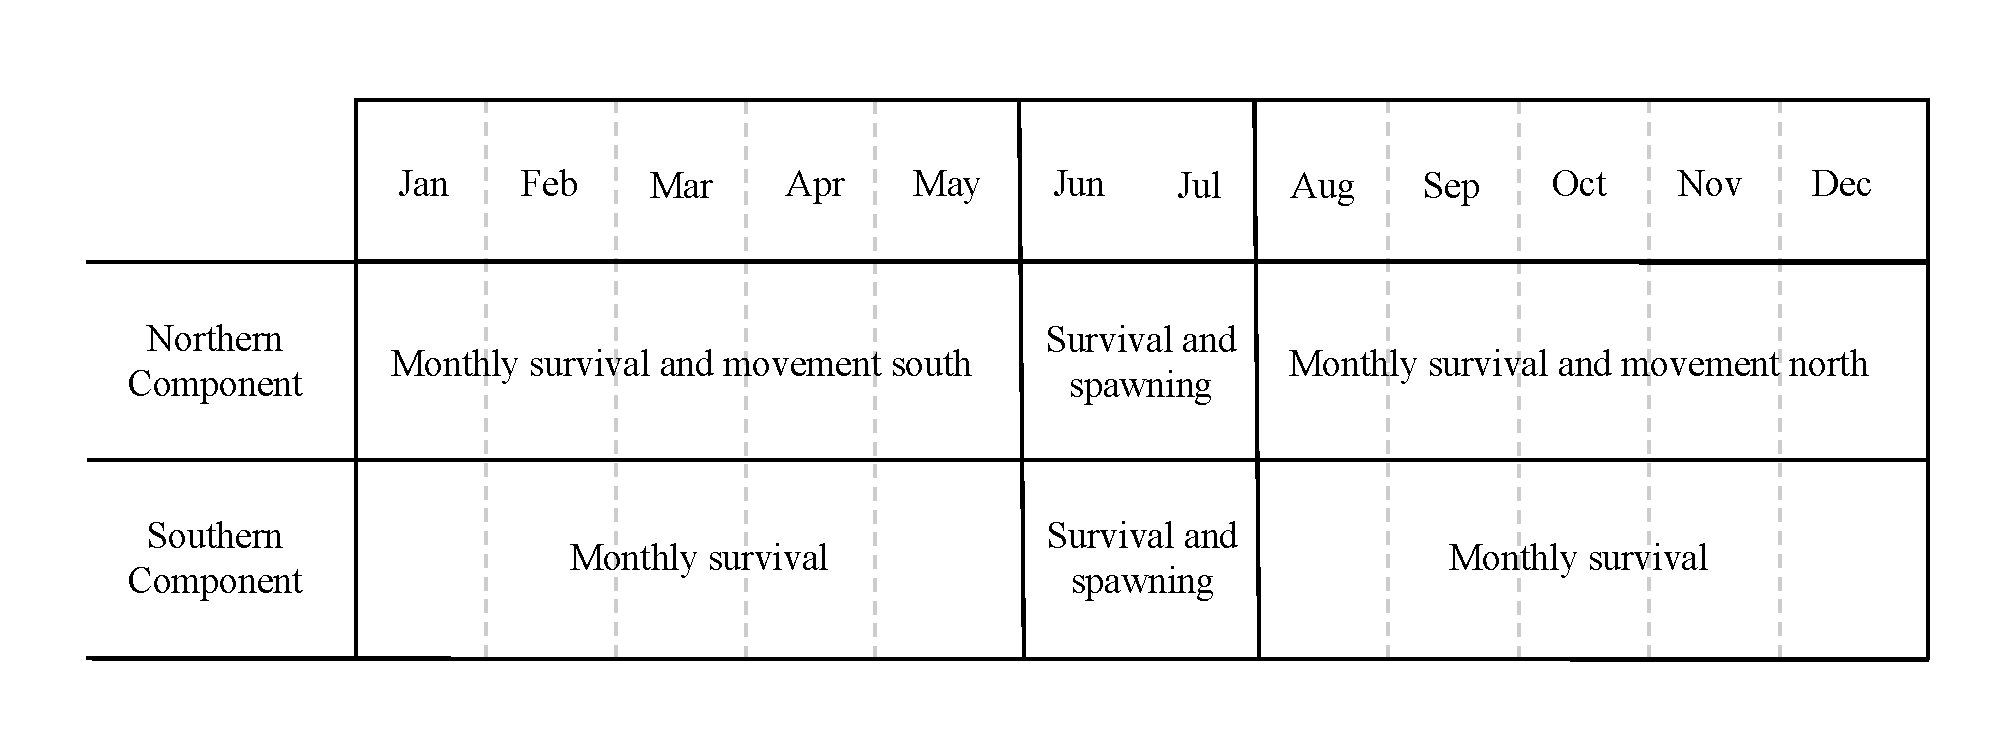
\includegraphics[width=0.8\linewidth]{bsb_movement_diagram} 

}

\caption{Diagram of intervals within the year and configuation of the dynamics of each component of the BSB population.}\label{fig:migration-diagram}
\end{figure}

\setcounter{table}{0}
\renewcommand\thetable{\arabic{table}}

\begin{landscape}\begin{table}

\caption{\label{tab:age-comp-sel-table}Configuration of Age composition likelihood, mean selectivity model, and selectivity random effects for each age composition data component.}
\centering
\begin{tabular}[t]{llll}
\toprule
Data component & Age Composition Likelihood & Mean Selectivity model & Random effects configuration\\
\midrule
North Commercial & Dirichlet-Multinomial & age-specific (flat-topped at ages > 3) & 2D-AR1 (age and year)\\
North Recreational & Logistic-normal (0s as missing) & age-specific (flat-topped at ages > 6) & 2D-AR1 (age and year)\\
South Commercial & Logistic-normal (AR1, 0s as missing) & logistic & None\\
South Recreational & Logistic-normal (AR1, 0s as missing) & logistic & None\\
North Recreational CPA & Logistic-normal (0s as missing) & age-specific (flat-topped at ages > 1) & AR1 (year)\\
\addlinespace
North VAST & Dirichlet-Multinomial & age-specific (flat-topped at ages > 4) & 2D-AR1 (age and year)\\
South Recreational CPA & Logistic-normal (AR1, 0s as missing) & age-specific (flat-topped at ages > 2) & None\\
South VAST & Logistic-normal (AR1, 0s as missing) & age-specific (flat-topped at ages > 1) & None\\
\bottomrule
\end{tabular}
\end{table}
\end{landscape}

\begin{table}

\caption{\label{tab:model-desc-table}Assumptions for temperature effects and random effects for age 1 natural mortality for each model.}
\centering
\begin{tabular}[t]{llll}
\toprule
\multicolumn{1}{c}{ } & \multicolumn{2}{c}{Temperature Effect} & \multicolumn{1}{c}{ } \\
\cmidrule(l{3pt}r{3pt}){2-3}
Model & North & South & $M$ at age 1 random effects\\
\midrule
$M_{0}$ & -- & -- & none\\
$M_{1}$ & Recruitment & -- & none\\
$M_{2}$ & -- & Recruitment & none\\
$M_{3}$ & Recruitment & Recruitment & none\\
$M_{4}$ & $M$ at age 1 & -- & none\\
\addlinespace
$M_{5}$ & -- & $M$ at age 1 & none\\
$M_{6}$ & $M$ at age 1 & $M$ at age 1 & none\\
$M_{7}$ & -- & -- & time-varying\\
$M_{8}$ & Recruitment & -- & time-varying\\
$M_{9}$ & -- & Recruitment & time-varying\\
\addlinespace
$M_{10}$ & Recruitment & Recruitment & time-varying\\
$M_{11}$ & $M$ at age 1 & -- & time-varying\\
$M_{12}$ & -- & $M$ at age 1 & time-varying\\
$M_{13}$ & $M$ at age 1 & $M$ at age 1 & time-varying\\
\bottomrule
\end{tabular}
\end{table}

\begin{table}

\caption{\label{tab:diff-aic-table}Difference between AIC and the lowest AIC for each model by retrospective peel.}
\centering
\begin{tabular}[t]{lrrrrrrrr}
\toprule
\multicolumn{1}{c}{ } & \multicolumn{8}{c}{Peel} \\
\cmidrule(l{3pt}r{3pt}){2-9}
Model & 0 & 1 & 2 & 3 & 4 & 5 & 6 & 7\\
\midrule
$M_{0}$ & 14.53 & 16.09 & 13.78 & 13.69 & 13.79 & 17.02 & 8.47 & 8.22\\
$M_{1}$ & 0.00 & 0.00 & 0.00 & 0.00 & 0.00 & 0.00 & 0.00 & 0.00\\
$M_{2}$ & 15.29 & 16.77 & 14.80 & 14.71 & 14.85 & 18.11 & 9.20 & 9.22\\
$M_{3}$ & 3.49 & 5.42 & 4.42 & 4.69 & 5.02 & 8.75 & 0.73 & 1.00\\
$M_{4}$ & 16.51 & 18.05 & 15.63 & 15.45 & 15.63 & 18.79 & 10.08 & 9.85\\
\addlinespace
$M_{5}$ & 16.09 & 17.51 & 15.30 & 15.16 & 15.29 & 18.41 & 9.86 & 9.71\\
$M_{6}$ & 18.07 & 19.46 & 17.14 & 16.92 & 17.12 & 20.18 & 11.46 & 11.33\\
$M_{7}$ & 17.05 & 18.48 & 15.57 & 14.96 & 15.39 & 18.19 & 9.71 & 9.42\\
$M_{8}$ & 5.02 & 6.87 & 4.90 & 4.66 & 5.28 & 8.59 & 0.98 & 0.99\\
$M_{9}$ & 17.82 & 19.17 & 16.59 & 15.98 & 16.45 & 19.28 & 10.44 & 10.43\\
\addlinespace
$M_{10}$ & 5.78 & 7.56 & 5.92 & 5.68 & 6.34 & 9.68 & 1.71 & 1.99\\
$M_{11}$ & 19.02 & 20.48 & 17.57 & 16.96 & 17.39 & 20.19 & 11.68 & 11.39\\
$M_{12}$ & 18.61 & 19.90 & 17.09 & 16.43 & 16.88 & 19.58 & 11.10 & 10.92\\
$M_{13}$ & 20.58 & 21.89 & 19.09 & 18.43 & 18.88 & 21.57 & 13.07 & 12.88\\
\bottomrule
\end{tabular}
\end{table}

\begin{table}

\caption{\label{tab:aic-wts-table}Model AIC weights for each retrospective peel.}
\centering
\begin{tabular}[t]{lrrrrrrrr}
\toprule
\multicolumn{1}{c}{ } & \multicolumn{8}{c}{Peel} \\
\cmidrule(l{3pt}r{3pt}){2-9}
Model & 0 & 1 & 2 & 3 & 4 & 5 & 6 & 7\\
\midrule
$M_{0}$ & 0.00 & 0.00 & 0.00 & 0.00 & 0.00 & 0.00 & 0.01 & 0.01\\
$M_{1}$ & 0.76 & 0.89 & 0.80 & 0.80 & 0.83 & 0.97 & 0.36 & 0.38\\
$M_{2}$ & 0.00 & 0.00 & 0.00 & 0.00 & 0.00 & 0.00 & 0.00 & 0.00\\
$M_{3}$ & 0.13 & 0.06 & 0.09 & 0.08 & 0.07 & 0.01 & 0.25 & 0.23\\
$M_{4}$ & 0.00 & 0.00 & 0.00 & 0.00 & 0.00 & 0.00 & 0.00 & 0.00\\
\addlinespace
$M_{5}$ & 0.00 & 0.00 & 0.00 & 0.00 & 0.00 & 0.00 & 0.00 & 0.00\\
$M_{6}$ & 0.00 & 0.00 & 0.00 & 0.00 & 0.00 & 0.00 & 0.00 & 0.00\\
$M_{7}$ & 0.00 & 0.00 & 0.00 & 0.00 & 0.00 & 0.00 & 0.00 & 0.00\\
$M_{8}$ & 0.06 & 0.03 & 0.07 & 0.08 & 0.06 & 0.01 & 0.22 & 0.23\\
$M_{9}$ & 0.00 & 0.00 & 0.00 & 0.00 & 0.00 & 0.00 & 0.00 & 0.00\\
\addlinespace
$M_{10}$ & 0.04 & 0.02 & 0.04 & 0.05 & 0.04 & 0.01 & 0.15 & 0.14\\
$M_{11}$ & 0.00 & 0.00 & 0.00 & 0.00 & 0.00 & 0.00 & 0.00 & 0.00\\
$M_{12}$ & 0.00 & 0.00 & 0.00 & 0.00 & 0.00 & 0.00 & 0.00 & 0.00\\
$M_{13}$ & 0.00 & 0.00 & 0.00 & 0.00 & 0.00 & 0.00 & 0.00 & 0.00\\
\bottomrule
\end{tabular}
\end{table}

\begin{table}

\caption{\label{tab:rho-table}Mohn's $\rho$ for SSB, R, average F at ages 6 and 7 in northern and southern regions.}
\centering
\begin{tabular}[t]{lrrrrrr}
\toprule
\multicolumn{1}{c}{ } & \multicolumn{2}{c}{SSB} & \multicolumn{2}{c}{Average F} & \multicolumn{2}{c}{Recruitment} \\
\cmidrule(l{3pt}r{3pt}){2-3} \cmidrule(l{3pt}r{3pt}){4-5} \cmidrule(l{3pt}r{3pt}){6-7}
Model & North & South & North & South & North & South\\
\midrule
$M_{0}$ & -0.031 & -0.026 & 0.032 & -0.043 & 0.211 & -0.007\\
$M_{1}$ & -0.040 & -0.023 & 0.041 & -0.048 & 0.181 & -0.024\\
$M_{2}$ & -0.031 & -0.027 & 0.032 & -0.043 & 0.211 & -0.007\\
$M_{3}$ & -0.031 & -0.027 & 0.031 & -0.043 & 0.193 & -0.007\\
$M_{4}$ & -0.032 & -0.026 & 0.032 & -0.044 & 0.268 & -0.006\\
\addlinespace
$M_{5}$ & -0.031 & -0.026 & 0.032 & -0.045 & 0.210 & -0.008\\
$M_{6}$ & -0.032 & -0.025 & 0.032 & -0.045 & 0.267 & -0.007\\
$M_{7}$ & -0.033 & -0.026 & 0.033 & -0.043 & 0.225 & -0.007\\
$M_{8}$ & -0.035 & -0.027 & 0.035 & -0.043 & 0.186 & -0.007\\
$M_{9}$ & -0.033 & -0.027 & 0.033 & -0.043 & 0.224 & -0.008\\
\addlinespace
$M_{10}$ & -0.035 & -0.027 & 0.035 & -0.043 & 0.186 & -0.008\\
$M_{11}$ & -0.032 & -0.026 & 0.032 & -0.044 & 0.253 & -0.007\\
$M_{12}$ & -0.033 & -0.026 & 0.033 & -0.045 & 0.224 & -0.008\\
$M_{13}$ & -0.032 & -0.025 & 0.032 & -0.045 & 0.253 & -0.008\\
\bottomrule
\end{tabular}
\end{table}
\clearpage

\hypertarget{supplemental-materials}{%
\section*{Supplemental Materials}\label{supplemental-materials}}
\addcontentsline{toc}{section}{Supplemental Materials}

\hypertarget{deriving-the-prior-distribution-for-movement-parameters}{%
\subsection*{Deriving the prior distribution for movement
parameters}\label{deriving-the-prior-distribution-for-movement-parameters}}
\addcontentsline{toc}{subsection}{Deriving the prior distribution for
movement parameters}

The working group fit a Stock Synthesis model (Methot and Wetzel 2013)
that included tagging data with 2 seasons (6 months each) and 2 regions
where a proportion \(\mu^*_1\) of the northern component moves to the
south in one season and some proportion \(\mu^*_{2\rightarrow 1}\) move
back to the south in the second season (NEFSC 2023). The seasonal
movement matrices for each season are \begin{equation*}
\boldsymbol{\mu}^*_{1} = 
  \begin{bmatrix}
     1-\mu^*_{1\rightarrow 2} & \mu^*_{1\rightarrow 2} \\
     0 & 1 \\
  \end{bmatrix}
\end{equation*} and \begin{equation*}
\boldsymbol{\mu}_{2} = 
  \begin{bmatrix}
     1 &  0 \\
     \mu^*_{2\rightarrow 1} & 1-\mu^*_{2\rightarrow 1} \\
  \end{bmatrix}.
\end{equation*}

To obtain estimates of movement proportions for the monthly intervals in
the WHAM model, the half-year movement matrices were converted to
monthly movement matrices by taking the root \(z_k\) of
\(\boldsymbol{\mu}^*_{k}\) which are defined by the number of months of
movement for each season (5 and 4, respectively). The roots of the
matrices are calculated using an eigen decomposition of the matrices
\[ \boldsymbol{\mu}_k =  \left(\boldsymbol{\mu}_k^*\right)^{z_k} = \mathbf{V}_k \mathbf{D}_k^{z_k} \mathbf{V}_k^{-1}\]
where \(z_1 = 1/5\) for and \(z_2 = 1/4\), and \(\mathbf{V}_{k}\) and
\(\mathbf{D}_{k}\) are the matrix of eigenvectors (columnwise) and the
diagonal matrix of corresponding eigenvalues of
\(\boldsymbol{\mu}^*_k\). The working group used a parametric bootstrap
approach to determine an appropriate standard deviation for the prior
distribution for the movement parameters. Stock Synthesis also estimates
parameters on a transformed scale, but different from WHAM:
\[\mu^*_{r\rightarrow r'} = \frac{1}{1 + 2e^{-x_{r\rightarrow r'}}}\]
The estimated parameters and standard errors from the Stock Synthesis
model were \(x_{1\rightarrow 2}=-1.44\) and \(x_{2\rightarrow 1}=1.94\)
and \(SE(x_{1\rightarrow 2})) = 0.21\) and
\(SE(x_{2\rightarrow 1})) = 0.37\). The resulting in the estimated
proportions were \(\mu^*_{1\rightarrow 2}=0.11\) and
\(\mu^*_{2\rightarrow 1}=0.78\).

In WHAM, an additive logit transformation is used which is simply a
logit transformation when there are only two regions: \[
\mu_{r\rightarrow r'} = \frac{1}{1+e^{-y_{r\rightarrow r'}}}.
\] We simulated 1000 values from a normal distribution with mean and
standard deviation defined by the parameter estimate and standard error
\(\tilde x_{{r\rightarrow r'},b} \sim N(x_{r\rightarrow r'}, SE(x_{r\rightarrow r'}))\)
from the Stock Synthesis model. For each simulated value we constructed
\(\tilde {\boldsymbol{\mu}}^*_{{r\rightarrow r'},b}\), took the
appropriate root and calculated inverse logit for
\(\tilde y_{{r\rightarrow r'},b}\). We calculated the mean and standard
deviation of the values \(y_{i,b}\). The mean values did not differ
meaningfully from the transformation of the original estimates
(\(y_{1\rightarrow 2} = -3.79\) and \(y_{2\rightarrow 1} = -0.79\)) and
the standard deviation was approximately 0.2 for both parameters.

\end{document}
